\chapter{Infraestructura}\label{cap.infraestructura}
En este capítulo se explican los principales ingredientes software en los que nos hemos apoyado  para desarrollar el trabajo. Tales como el simulador Gazebo (con el cual podemos simular las acciones que realizaría un robot en un mundo determinado), el entorno JdeRobot, la librería de OpenCV (empleada en todo lo relacionado con el tratamiento de imagen), PyQt (para el desarrollo de la interfaz gráfica) y Python como lenguaje de programación.

\section{Simulador Gazebo}
Gazebo es un simulador usado en robótica que permite emular diversos escenarios tridimensionales donde probar nuestro software. A la hora de realizar el software robótico es necesario hacer pruebas, las cuales saldrían muy caras si se probarán en robots reales (podría no funcionar correctamente y que nuestro robot se rompiera). Por esta razón es muy útil el empleo de simuladores, pues podemos realizar las pruebas que queramos sin peligro de que nuestro robot salga averiado. Con los simuladores se pueden diseñar robots y escenarios realistas donde ejecutar algoritmos de percepción y control.

\begin{figure}[H]
  \begin{center}
    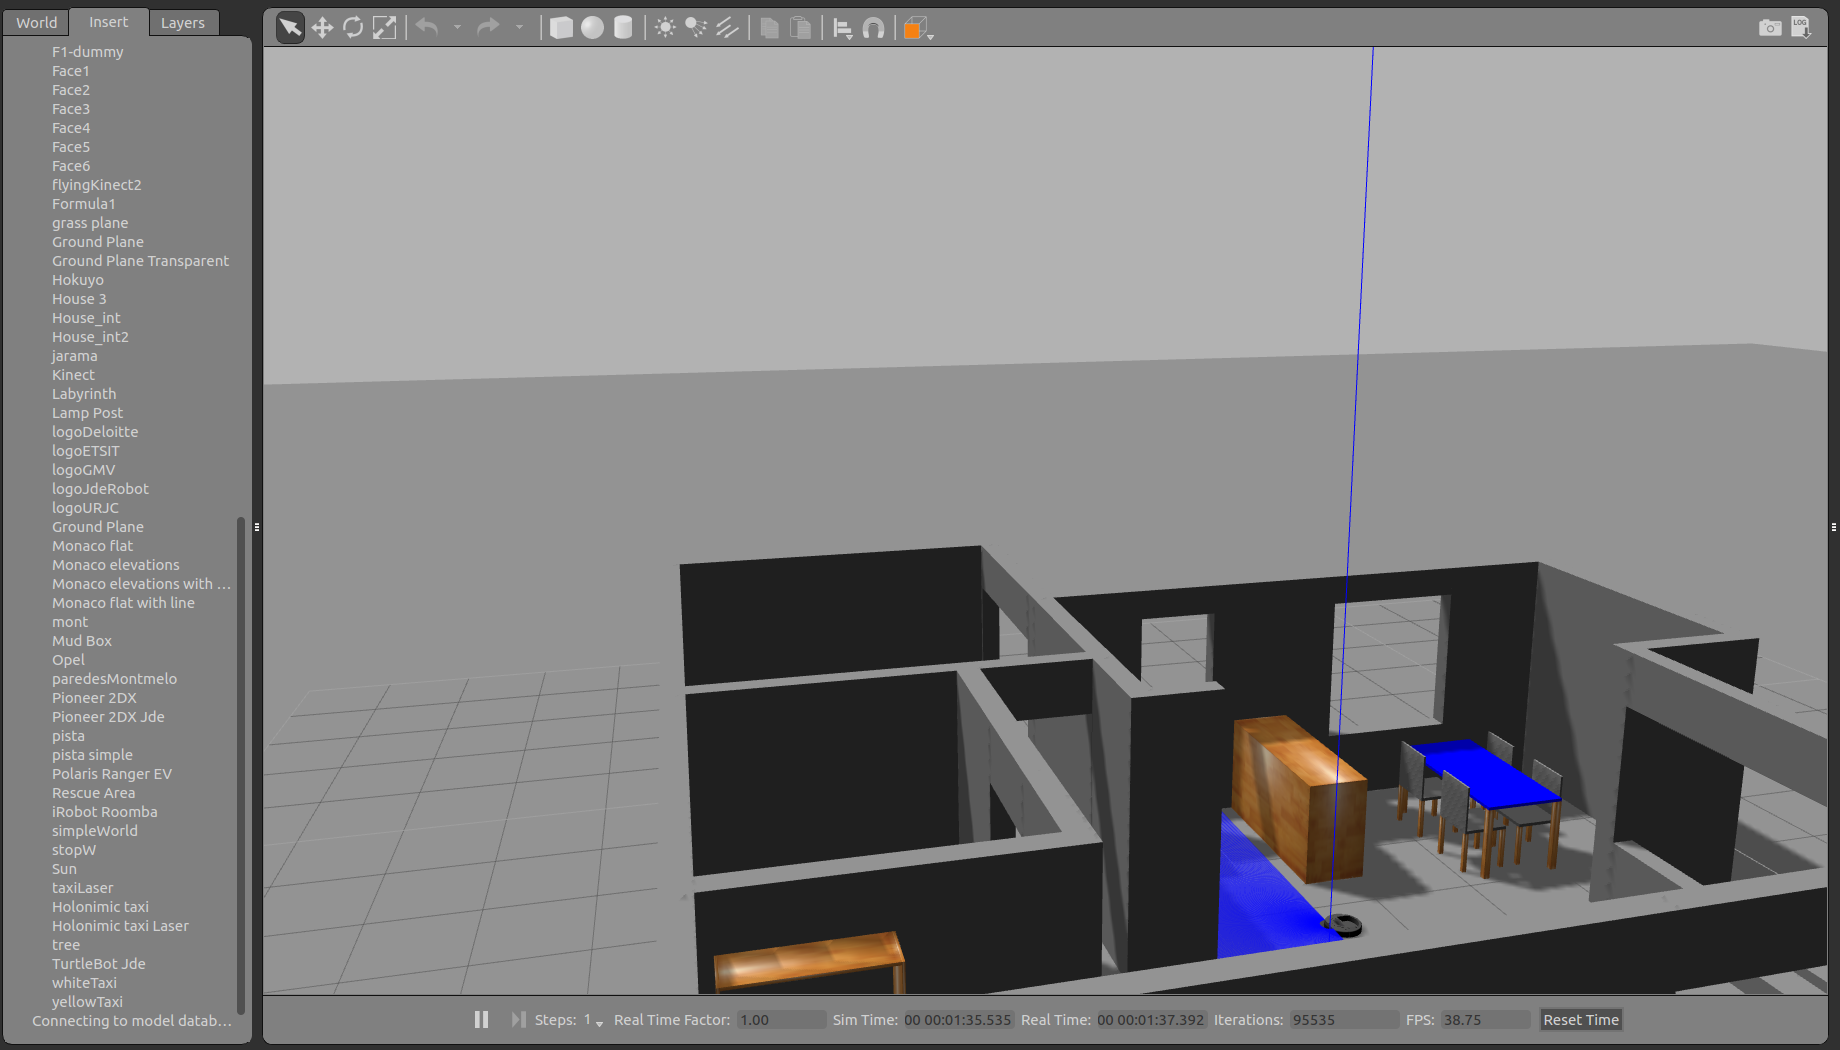
\includegraphics[width=0.7\textwidth]{figures/Infraestructura/gazebo.png}
		\caption{Simulador Gazebo}
		\label{fig.gazebo}
		\end{center}
\end{figure}

Gazebo es un programa de código abierto distribuido bajo licencia de Apache 2.0. Es uno de los ejes del entorno docente de JdeRobot-Academy.  Se emplea en el desarrollo de aplicaciones robóticas y en inteligencia artificial. Es capaz de simular robots, objetos y sensores en entornos complejos de interior y exterior. Tiene gráficos de gran calidad y un robusto motor de físicas (masa del robot, rozamiento, inercia, amortiguamiento, etc.). Fue elegido para realizar el DARPA Robotics Challenge (2012--2015) y está mantenido por la Fundación Robótica de Código Abierto (OSRF).\\

En este trabajo se emplea la versión 7 de Gazebo \footnote{\url{http://gazebosim.org/blog/gazebo7}}.  Gracias a Gazebo se pueden incluir texturas, luces y sombras en los escenarios, así como simular la física como por ejemplo choques, empujes, gravedad, etc. Además, incluye diversos sensores, como pueden ser cámaras y láseres, los cuales podrán ser incorporados en los robots que empleemos. Todo ello hace que sea una herramienta muy potente y de gran ayuda en robótica.\\

Los mundos simulados con Gazebo son mundos 3D, que se cargan a partir de ficheros con extensión ``.world''. Son ficheros \acrfull{xml} definidos en el lenguaje \acrfull{sdf}. Este lenguaje contiene una descripción completa de todos los elementos que tiene el mundo y los robots, incluyendo:

\begin{itemize}
\item Escena: Luz ambiente, propiedades del cielo, sombras, etc.
\item Mundo: Representa el mundo como un conjunto de modelos, \textit{plugins} y propiedades físicas.
\item Modelo: Articulaciones, objetos de colisión, sensores, etc.
\item Físicas: Gravedad, motor físico, paso del tiempo, colisiones, inercias, etc.
\item Plugins: Sobre un mundo, modelo o sensor.
\item Luz: Los puntos y origen de la luz.
\end{itemize}

Las etiquetas empleadas en el fichero para representar estos elementos son: Scene, World, Model, Physics, Plugin, y Light.\\

Los modelos de robots que se emplean en la simulación son creados mediante algún programa de modelado 3D (Blender, Sketchup…). Estos robots simulados necesitan ser dotados de inteligencia para lo cual se emplean los \textit{plugins}. Estos \textit{plugins} pueden dotar al robot de inteligencia u ofrecer la información de sus sensores a aplicaciones externas y recibir de éstas comandos para los actuadores de los robots.


\section{Entorno JdeRobot}
JdeRobot \footnote{\url{http://jderobot.org/Main_Page}} es un \textit{middleware} de software libre para el desarrollo de aplicaciones con robots y visión artificial. Esta plataforma fue creada por el Grupo de Robótica de la Universidad Rey Juan Carlos en 2003 y está licenciada como GPLv3 \footnote{\url{https://www.gnu.org/licenses/quick-guide-gplv3.html}}.\\

Está desarrollado en C y C++, aunque contiene componentes desarrollados en lenguajes como Python y JavaScript. El entorno que ofrece está basado en componentes, los cuales se ejecutan como procesos. Dichos componentes interoperan entre sí a través del \textit{middleware} de comunicaciones \acrshort{ice} o de \acrshort{ros} messages. Tanto \acrshort{ice} como \acrshort{ros}-messages permiten la interoperación entre los componentes incluso estando desarrollados en diferentes lenguajes.\\

Es capaz de llevar a cabo diferentes tareas en tiempo real de forma sencilla. Cada componente \textit{driver} está asociado a un dispositivo hardware del robot, un sensor o actuador e incluye funciones para poder emplearlo. Esto simplifica el acceso a los diferentes componentes hardware, ya que con una simple función se puede acceder a ellos.\\

Las aplicaciones constan de uno o varios componentes. Los que interactúan directamente con los sensores y actuadores del robot se llaman \textit{drivers}, que son los encargados de controlar que los robots reciben órdenes a través de interfaces \acrshort{ice} o \acrshort{ros} messages. Otros llevan en su código las funciones perceptivas, procesamiento de señales o la lógica de control e inteligencia del robot. En la siguiente imagen se puede ver un ejemplo de esta comunicación con un AR Drone empleando interfaces \acrshort{ice}. La misma lógica de comportamiento se puede conectar al \textit{driver} del drone real o al \textit{driver} del drone simulado, basta con cambiar la configuración.

\begin{figure}[H]
  \begin{center}
    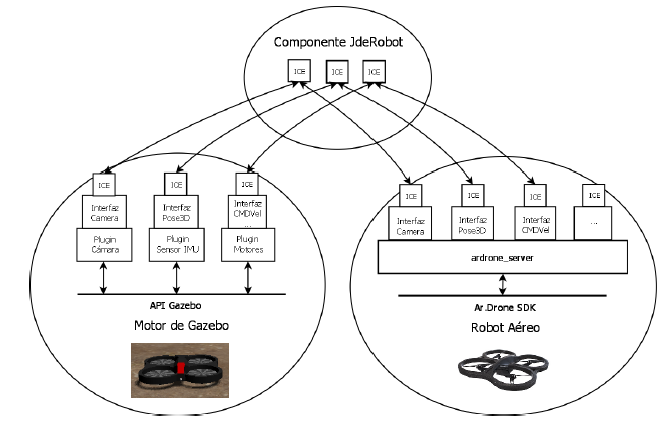
\includegraphics[width=0.7\textwidth]{figures/Infraestructura/jderobot.png}
		\caption{Ejemplo de componentes JdeRobot }
		\label{fig.jderobot}
		\end{center}
\end{figure}

Esta plataforma soporta gran variedad de dispositivos como el cuadricóptero AR Drone de Parrot, el robot Pioneer de MobileRobotics Inc., el robot Kobuki de Yujin Robot, el humanoide NAO de Aldebaran Robotics, cámaras firewire, USB e IP, los escáneres laser LMS de SICK y URG de Hokuyo, los simuladores Stage y Gazebo, sensores de profundidad como Kinect y otros dispositivos X10 de dómotica. A parte de todo esto, tiene soporte para software externo como OpenCV, OpenGL, XForms, GTK, Player y GSL.   \\

En el desarrollo de las prácticas de este TFG se empleará la versión 5.5.2 de JdeRobot, ya que es la última versión estable.


\section{Python}
Python \footnote{\url{https://www.python.org/}} es un lenguaje de programación fácil de aprender y de alto nivel. Su creador fue Guido van Rossum, un investigador holandés que trabajaba en el centro de investigación CWI (Centrum Wiskunde \& Informatica). La primera versión surgió en 1991 pero no fue publicado hasta tres años después. Guido dio el nombre de Python en honor a la serie de televisión \textit{Monty Python’s Flying Circus}.\\


Python incluye orientación a objetos, manejo de excepciones, listas, diccionarios, etc. A pesar de todo lo que soporta, se creó con el objetivo de que fuera un lenguaje sencillo de entender, sin perder las funcionalidades que pueden ofrecer lenguajes complejos tales como C.\\

Actualmente Python es un lenguaje de código abierto administrado por Python Software Foundation. Incluye módulos que permiten la entrada y salida de ficheros, \textit{sockets}, llamadas al sistema e incluso interfaces gráficas como Qt. Además, permite dividir el programa en módulos reutilizables y no es necesario compilarlo, pues es interpretado. Es uno de los ejes de JdeRobot-Academy.\\

La última versión ofrecida por Python Software Foundation es la 3.6.2 , pero en nuestro caso se empleará la 2.7.12 por compatibilidad con JdeRobot 5.5.2, que a su vez sigue en esa versión de Python para ser compatible con \acrshort{ros} Kinetic. El código en el que están escritos los componentes académicos y las soluciones es Python.

\section{Biblioteca OpenCV}
OpenCV \footnote{\url{http://opencv.org/}} es una librería de código abierto desarrollada inicialmente por Intel y publicada bajo licencia de BSD. Esta librería implementa gran variedad de herramientas para la interpretación de la imagen. Sus siglas provienen de los términos anglosajones ``Open Source Computer Vision Library'', y está orientada a aplicaciones de visión por computador en tiempo real.  \\

Esta librería puede ser usada en MacOS, Windows, Android y Linux, y existen versiones para C\#, Python y Java, a pesar de que originalmente era una librería en C/C++. Además, hay interfaces en desarrollo para Ruby, Matlab y otros lenguajes.\\

OpenCV principalmente implementa algoritmos para las técnicas de calibración, detección de rasgos, para el rastreo, análisis de la forma, análisis del movimiento, reconstrucción 3D, segmentación de objetos y reconocimiento. Los algoritmos se basan en estructuras de datos flexibles acopladas con estructuras IPL (Intel Image Processing Library), aprovechándose de la arquitectura de Intel en la optimización de más de la mitad de las funciones.  \\

Fue diseñado para tener una alta eficiencia computacional. Está escrito en C y puede aprovechar las ventajas de los procesadores multinúcleo. La biblioteca de OpenCV contiene más de 500 funciones que abarcan muchas áreas de la visión artificial. También tiene una librería de aprendizaje automático (MLL, Machine Learning Library) destinada al reconocimiento y agrupación de patrones estadísticos. 

\begin{figure}[H]
  \begin{center}
    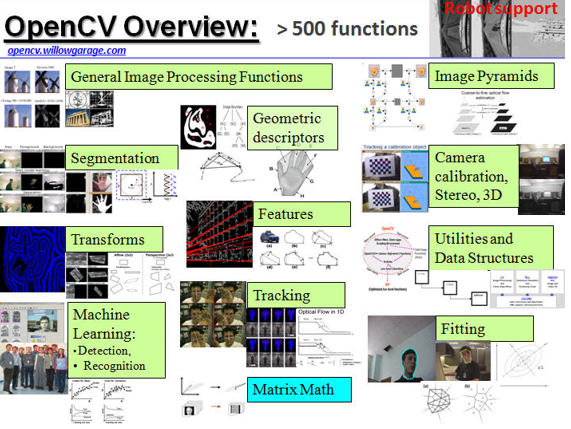
\includegraphics[width=0.6\textwidth]{figures/Infraestructura/opencv.png}
		\caption{Funciones de OpenCV }
		\label{fig.opencv}
		\end{center}
\end{figure}

OpenCV está compuesto por numerosas librerías con las cuales podemos manejar estructuras de datos, detectar bordes y esquinas, escalar o rotar imágenes, modificar el espacio de color de una imagen, realizar emparejamiento, detectar líneas y círculos, tratar objetos en 3D, crear ventanas y asociar eventos a dichas ventanas, etc. Incorpora funciones básicas para modelar el fondo, sustraer dicho fondo, generar imágenes de movimiento MHI (Motion History Images), etc. Además, incluye funciones para determinar dónde hubo movimiento y en qué dirección. \\


Desde su aparición OpenCV ha sido usado en numerosas aplicaciones. Hay una gran cantidad de empresas y centros de investigación que emplean estas técnicas como IBM, Microsoft, Intel, SONY, Siemens, Google, Stanford, MIT, CMU, Cambridge e INRIA.\\

En este trabajo se ha empleado la versión 3.2 de OpenCV en Python. Esta librería se empleará para realizar todo lo relacionado con el tratamiento de imágenes. Con ella se extraerán datos que puedan emplearse a la hora de tomar decisiones para que los robots funcionen correctamente.

\section{PyQt}
PyQt~\cite{python1}~\cite{pqt} es un conjunto de enlaces Python para el conjunto de herramientas Qt, las cuales se emplean para el desarrollo de interfaces gráficas. Fue desarrollado por Riverbank Computing Ltd y es soportado por Windows, Linux, Mac OS/X, iOS y Android.\\

Qt es un entorno multiplataforma orientado a objetos desarrollado en C++  que permite desarrollar interfaces gráficas e incluye \textit{sockets}, hilos, Unicode, bases de datos SQL, etc. PyQt combina todas las ventajas de Qt y Python, pues permite emplear todas las funcionalidades ofrecidas por Qt con un lenguaje de programación tan sencillo como Python.\\

En este proyecto se ha empleado la versión 5 de PyQt. PyQt5 es un conjunto de enlaces Python para Qt5, disponible en Python 2.x y 3.x. Tiene más de 620 clases y 6000 funciones y métodos. PyQt5 dispone de una licencia dual, es decir, los desarrolladores pueden elegir entre una licencia GPL (General Public Licence) o una licencia comercial. \\

La interfaz gráfica de los componentes académicos creados en las prácticas está escrita usando PyQt. Las clases de PyQt5 se dividen en ciertos módulos, tales como QtCore, QtGui, QtWidgets, QtXml, QtSql, etc. En las prácticas desarrolladas se ha hecho uso de los siguientes módulos:

\begin{itemize}
\item QtCore: contiene las funcionalidades principales que no tienen que ver con la \acrshort{gui}. Este módulo se emplea para trabajar con archivos, diferentes tipos de datos, hilos, procesos, url, etc.
\item QtGui: contiene clases para el desarrollo de ventanas, gráficos 2D, imágenes y texto.
\item QtWidgets: dispone de clases que proporcionan un conjunto de elementos de interfaz de usuario para crear GUIs clásicas de escritorio. 
\end{itemize}